%\documentclass[twocolumn]{article}
%\usepackage[utf8]{inputenc}
%\documentclass[10pt,journal,onecolumn]{IEEEtran}
%\documentclass[10pt,journal,compsoc]{IEEEtran}
\documentclass[10pt, journal, letterpaper]{IEEEtran}
%\documentclass[10pt,journal,compsoc]{IEEEtran}


% NB hyperref package may need to be commented for Latex upload
\usepackage{cite}
%\ifCLASSOPTIONcompsoc
%\ifCLASSINFOpdf
% \usepackage[pdftex]{graphicx}
% declare the path(s) where your graphic files are
% \graphicspath{{../pdf/}{../jpeg/}}
% and their extensions so you won't have to specify these with
% every instance of \includegraphics
% \DeclareGraphicsExtensions{.pdf,.jpeg,.png}
%  \usepackage[nocompress]{cite}
%  \else
% normal IEEE
%  \usepackage{cite}
%  \fi

%  \ifCLASSINFOpdf

%  \else
%\fi
%important package
\usepackage{multirow} 
\usepackage{algpseudocode}
\usepackage{algorithm}
\usepackage{rotating}
\usepackage{kantlipsum} %with the next two command (commath, allowdisplaybreaks) -> allow to break the formulas along the pages
\usepackage{commath}
\allowdisplaybreaks
\usepackage{mathtools}  %with the next command adjust the vertical space between formulas
%\setlength{\jot}{5pt}
%\usepackage{ragged2e}   %if add \justify at each line, that line would be justified. This is used because the abstract of transaction style is not justified  ---- it is not compatible with twocolumn-IEEETrans
%not important
\usepackage{verbatim}
\usepackage{xr-hyper} 
\usepackage{enumitem}
\usepackage{multirow}
\usepackage[table,xcdraw]{xcolor}
\usepackage{array,arydshln}
\usepackage{graphicx,booktabs}
\usepackage{longtable}
%strikethrough not working when nested in a definition
%\usepackage[normalem]{ulem}
%\usepackage{soul}
%\usepackage{fullpage} 
%%%%%%%%%%%%%%%%%%%%%%%%%%%%%%%%%%%%%%%%%%%%%%%%%%%%%%%%%%%%%%%%%%%%%%%%%%%%%
% hyperref package may need to be commented for Latex upload
%\usepackage[pdfusetitle, pdfauthor={Michael Shell, My institution}]{hyperref}
%%%%%%%%%%%%%%%%%%%%%%%%%%%%%%%%%%%%%%%%%%%%%%%%%%%%%%%%%%%%%%%%%%%%%%%%%%%%%
\usepackage{balance}
\usepackage{flushend}
\usepackage{epstopdf}
\usepackage{wrapfig}
\usepackage{latexsym}
\usepackage{amssymb}
\usepackage{amsthm}
\usepackage{amsfonts}
\usepackage{amsmath} %[cmex10]
%\usepackage{flushend} %********************* This package has a bug: Do no include it
\usepackage{graphicx}
\usepackage{latexsym}
\usepackage{booktabs}
\usepackage[style=base]{caption}
\usepackage{subcaption} %******************* This package has conflict with sufig and subfigure
%\usepackage{subfigure}
%\usepackage{subfig}
\usepackage{breqn}
\newtheorem{thm}{Property}
\newtheorem{thm1}{Theorem}
\newtheorem{thm3}{Proposition}
\newtheorem{thm5}{Remark}
\newtheorem{thm7}{Lemma}
\algnewcommand\algorithmicinput{\textbf{INPUT:}}
\algnewcommand\INPUT{\item[\algorithmicinput]}
\algnewcommand\algorithmicoutput{\textbf{OUTPUT:}}
\algnewcommand\OUTPUT{\item[\algorithmicoutput]}
\usepackage[table]{xcolor}
%\usepackage[dvipsnames]{xcolor}
%\usepackage[cmyk]{xcolor}
%\usepackage{natbib}
\usepackage{graphicx}
\usepackage{mathtools}
\usepackage{enumitem,kantlipsum}
\usepackage{adjustbox}
% change the width and height of rows and columns in Tables
\usepackage[thinlines]{easytable}

\algdef{SE}[DOWHILE]{Do}{doWhile}{\algorithmicdo}[1]{\algorithmicwhile\ #1}
\makeatletter
\algnewcommand{\LineComment}[1]{\Statex \hskip\ALG@thistlm \texttt{#1}}
\makeatother
\newcommand{\export}{Exportation\xspace}
\newcommand{\move}{Move\xspace}
\newcommand{\ouralgorithm}{GPE\xspace} %%Green path exportation

\newlength\mylength
\setlength\mylength{\dimexpr.13\columnwidth-1\tabcolsep-0.2\arrayrulewidth\relax}
\usepackage{color}
% we need a better fix for this, see https://tex.stackexchange.com/questions/64298/error-with-xcolor-package
\colorlet{BLUE}{blue}
\usepackage{colortbl}
\definecolor{LightCyan}{RGB}{155, 227, 247}
%\captionsetup[figure]{belowskip=-8pt}
%in test

%\usepackage{nomencl}
%\makenomenclature
%% This code creates the groups
% -----------------------------------------
%\usepackage{etoolbox}
%\renewcommand\nomgroup[1]{%
%	\item[\bfseries
%	\ifstrequal{#1}{P}{Parameters}{%
%		\ifstrequal{#1}{V}{Variables}{%
%			\ifstrequal{#1}{I}{Indices}{%
%				\ifstrequal{#1}{B}{Binary~Variables}{}}}}%
%	]}

%DOUBLE QUOTATION COMMAND
\newcommand{\dq}[1]{``#1''}

% To remove all comments, comment out the definition and use the commented-out
% empty definition below
% otherwise you can comment the line \commentsontrue 
\newcommand{\commentBy}[3]{\textcolor{#1}{\textbf{#2:} #3}}
%\newcommand{\commentBy}[3]{\ignorespaces}

\newif\ifcommentson
%uncomment the line below to show comments
\commentsontrue

\newcommand{\ste}[1]{\ifcommentson \commentBy{blue}{SS}{#1} \fi}
%\newcommand{\lc}[1]{\ifcommentson \commentBy{blue}{LC}{#1} \fi}
\newcommand{\mm}[1]{\ifcommentson \commentBy{orange}{MM}{#1} \fi}

\newif\ifextended
\newif\ifshortver

%%% Show only short version in black
%%%        \shorvetrue 
%%%        %\extendedtrue 

%%% Show only extended version in black
%%%        %\shorvetrue 
%%%        \extendedtrue 

%%% Show short version in blue and extended version in purple
%%%        \shorvetrue 
%%%        \extendedtrue 

\shortvertrue
%\extendedtrue

\newcommand{\extended}[1]{\ifextended \ifshortver \textcolor{purple}{#1} \else \textcolor{black}{#1} \fi  \fi}
\newcommand{\shortver}[1]{\ifshortver \ifextended \textcolor{blue}{#1} \else \textcolor{black}{#1} \fi \fi}

%\newcommand{\optional}[1]{#1}
%\newcommand{\optional}[1]{\textcolor{Orange}{#1}}
\newcommand{\optional}[1]{\ignorespaces}


\newif\ifrevisionactive
\newif\ifshowdeleted
\revisionactivetrue
%\showdeletedtrue

\newcommand{\revised}[1]{\ifrevisionactive \textcolor{blue}{#1} \else \textcolor{black}{#1} \fi}

%\newcommand{\deleted}[1]{\ifrevisionactive \ifshowdeleted \textcolor{red}{\sout{#1}} \else \fi \fi}
\newcommand{\deleted}[1]{\ifrevisionactive \ifshowdeleted \textcolor{orange}{#1} \else \fi \fi}


% correct bad hyphenation here
\hyphenation{net-works mo-ni-to-ring par-ti-cu-lar pe-ri-o-di-cal-ly mi-ni-mi-zing va-ria-tions de-li-ve-red per-ri-o-di-cal-ly}


\newcommand\linearFigSze{0.48}
\newcommand\histFigSze{0.48}
\newcommand\boxFigSze{1}

\newcommand{\red}[1]{\textcolor{red}{#1}}

\begin{document}
\title{GEANT: Traffic Pattern, Break Down to Elements, and COVID-19 impacts}
\author{}
%\date{October 2018}
\maketitle	
\begin{abstract}
\end{abstract}	
\begin{IEEEkeywords} 
    Passive Network Monitoring;
\end{IEEEkeywords}

\section{Introduction}
INTRODUCTION TO GEANT.

DATA-SET WE USED.

A BRIEF POINT TO OUR FINDINGS.

\section{Impact of New Year Holidays on GEANT}
In this section, we look into the impact of 'new year holidays' on the GEANT traffic pattern. To this end, we do sampling over two different time-periods, one in Dec long away from new year holidays (2019/12/09 - 2019/12/15) and the other one during new year holidays (2019/12/30 - 2020/01/05). We first analyse the total traffic throughput in terms of byte per second (bps) and flow per second (fps). Thereafter, we break-down the traffic into its academic and business elements and their pattern during the week. After that, the top NRENs generating and receiving traffic is discussed to investigate the impact of new year holidays on top NRENs pattern. The same process is followed for top ASes generating and receiving traffic.

\subsection{Total Traffic Throughput}
Fig.~\ref{fig:datarate_BCH_CH} show the impact of new year holidays on the total data rate throughput. There is an evident pattern during the week long before new year holidays. From midnight
\begin{figure}
    \begin{subfigure}{\linearFigSze\textwidth}
          \centering
          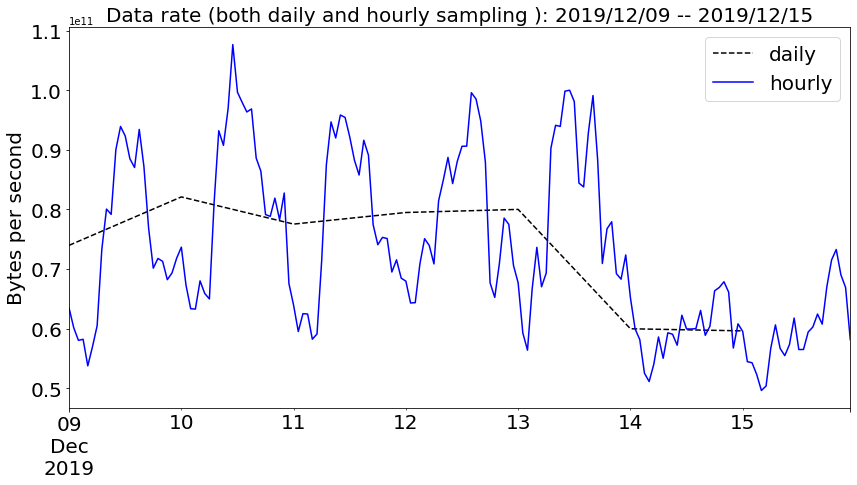
\includegraphics[width=\columnwidth]{img/BCH2_byterate.png}
          \caption{Data-rate before new year holidays}
          \label{fig:BCH2_bps}
    \end{subfigure}
    \begin{subfigure}{\linearFigSze\textwidth}
          \centering
          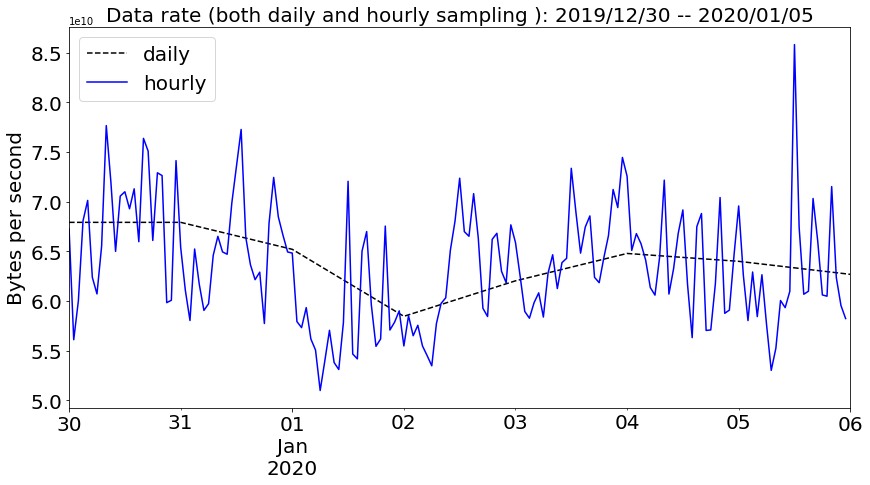
\includegraphics[width=\columnwidth]{img/CH2_byterate.png}
          \caption{Data-rate during new year holidays}
          \label{fig:CH2_bps}
    \end{subfigure}
    \caption{Impact of new year holidays on data rate}
    \label{fig:datarate_BCH_CH}
\end{figure}

\begin{figure}
    \begin{subfigure}{\linearFigSze\textwidth}
          \centering
          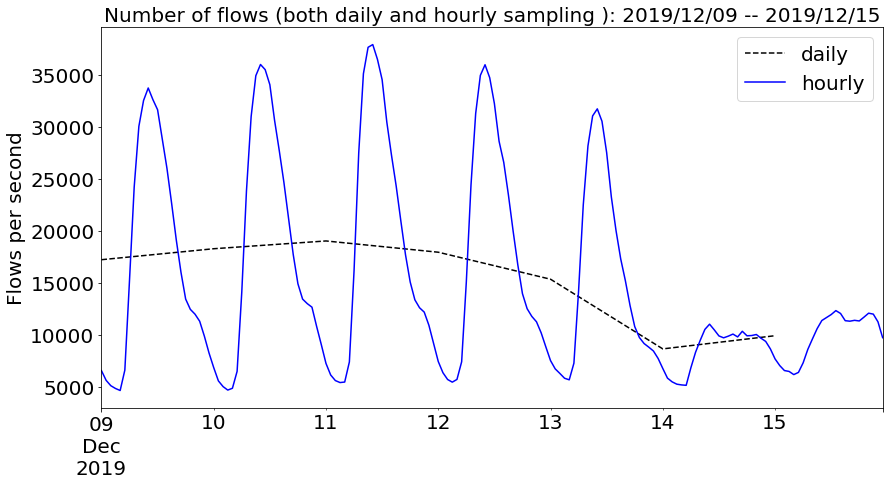
\includegraphics[width=\columnwidth]{img/BCH2_flowrate.png}
          \caption{Flow-rate before new year holidays}
          \label{fig:BCH2_fps}
    \end{subfigure}
    \begin{subfigure}{\linearFigSze\textwidth}
          \centering
          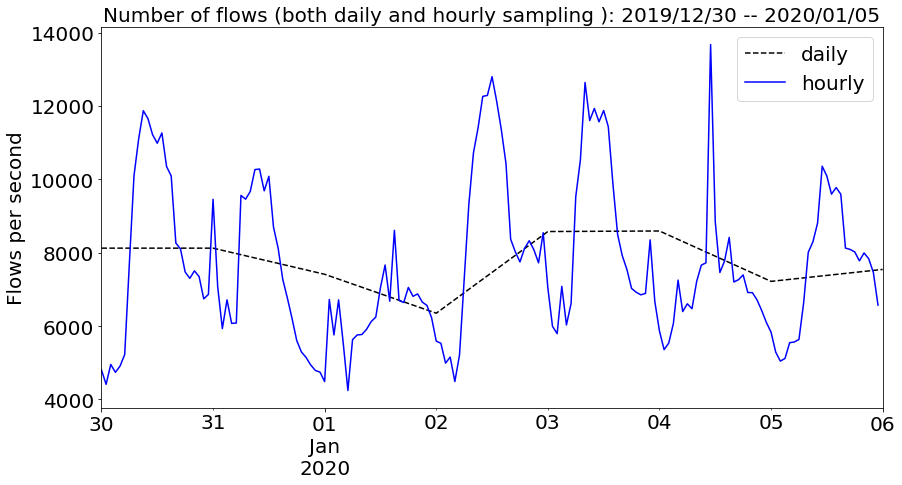
\includegraphics[width=\columnwidth]{img/CH2_flowrate.png}
          \caption{Flow-rate during new year holidays}
          \label{fig:CH2_fps}
    \end{subfigure}
    \caption{Impact of new year holidays on flow rate}
    \label{fig:flowrate_BCH_CH}
\end{figure}

\subsection{Academic and Business Traffic}
\begin{figure}
    \begin{subfigure}{\linearFigSze\textwidth}
          \centering
          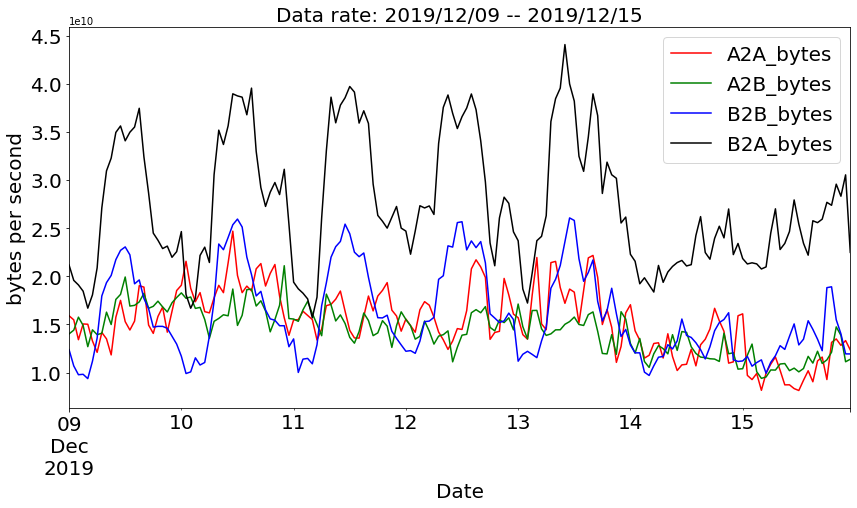
\includegraphics[width=\columnwidth]{img/BCH2_acaBus_bps.png}
          \caption{Data-rate before new year holidays}
          \label{fig:BCH2_acaBus_bps}
    \end{subfigure}
    \begin{subfigure}{\linearFigSze\textwidth}
          \centering
          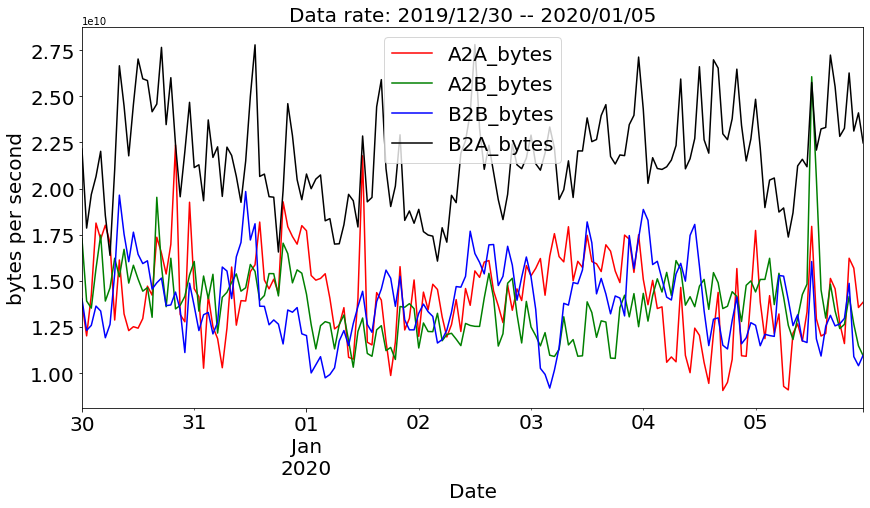
\includegraphics[width=\columnwidth]{img/CH2_acaBus_bps.png}
          \caption{Data-rate during new year holidays}
          \label{fig:CH2_acaBus_bps}
    \end{subfigure}
    \caption{Impact of new year holidays on data rate of academic and business traffic}
    \label{fig:datarate_acaBus_BCH_CH}
\end{figure}

\begin{figure}
    \begin{subfigure}{\linearFigSze\textwidth}
          \centering
          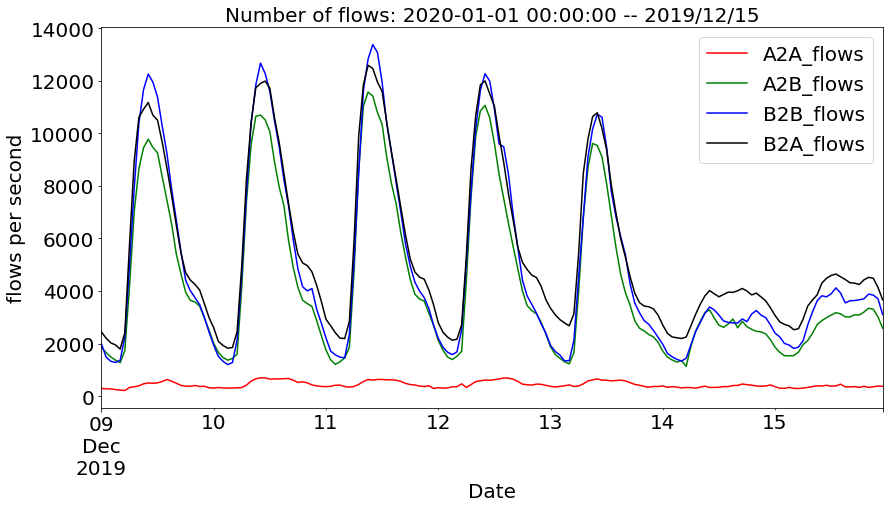
\includegraphics[width=\columnwidth]{img/BCH2_acaBus_fps.png}
          \caption{Flow-rate before new year holidays}
          \label{fig:BCH2_acaBus_fps}
    \end{subfigure}
    \begin{subfigure}{\linearFigSze\textwidth}
          \centering
          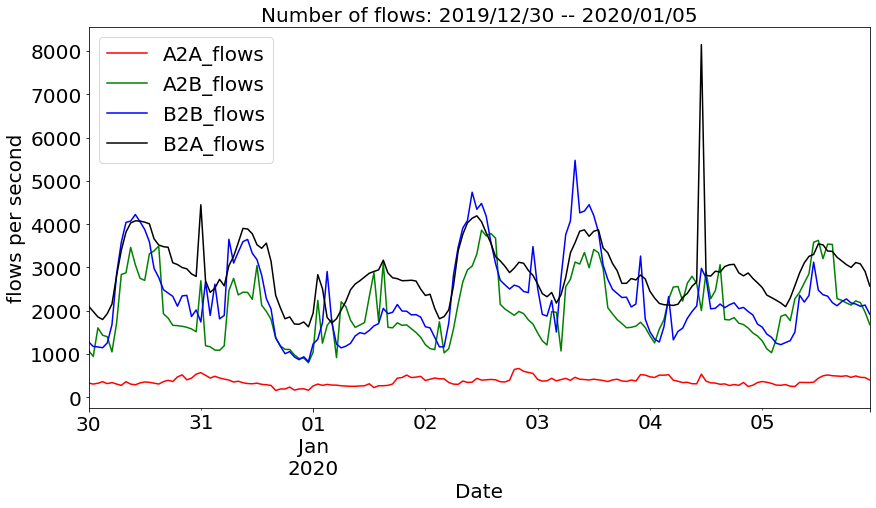
\includegraphics[width=\columnwidth]{img/CH2_acaBus_fps.png}
          \caption{Flow-rate during new year holidays}
          \label{fig:CH2_acaBus_fps}
    \end{subfigure}
    \caption{Impact of new year holidays on flow rate of academic and business traffic}
    \label{fig:flowrate_acaBus_BCH_CH}
\end{figure}

\subsection{NRENs Traffic}

\subsection{Top ASes}
\begin{figure}
    \begin{subfigure}{\linearFigSze\textwidth}
          \centering
          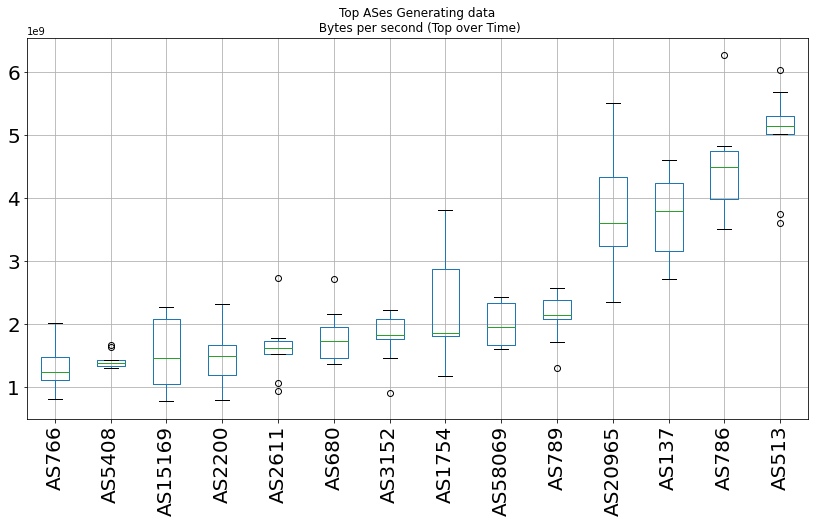
\includegraphics[width=\columnwidth]{img/BCH2_top14AS_generating_bps.png}
          \caption{Top 14 ASes generating traffic before new year holidays}
          \label{fig:BCH2_topAS_gen_bps}
    \end{subfigure}
    \begin{subfigure}{\linearFigSze\textwidth}
          \centering
          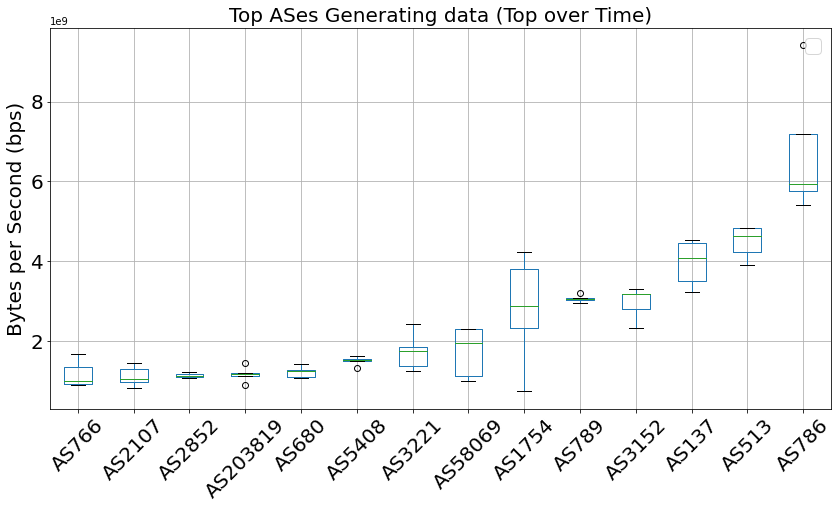
\includegraphics[width=\columnwidth]{img/CH2_top14AS_generating_bps.png}
          \caption{Top 14 ASes generating traffic during new year holidays}
          \label{fig:CH2_topAS_gen_bps}
    \end{subfigure}
    \caption{Impact of new year holidays on data rate of academic and business traffic}
    \label{fig:topAS_gen_BCH_CH}
\end{figure}

\begin{figure}
    \begin{subfigure}{\linearFigSze\textwidth}
          \centering
          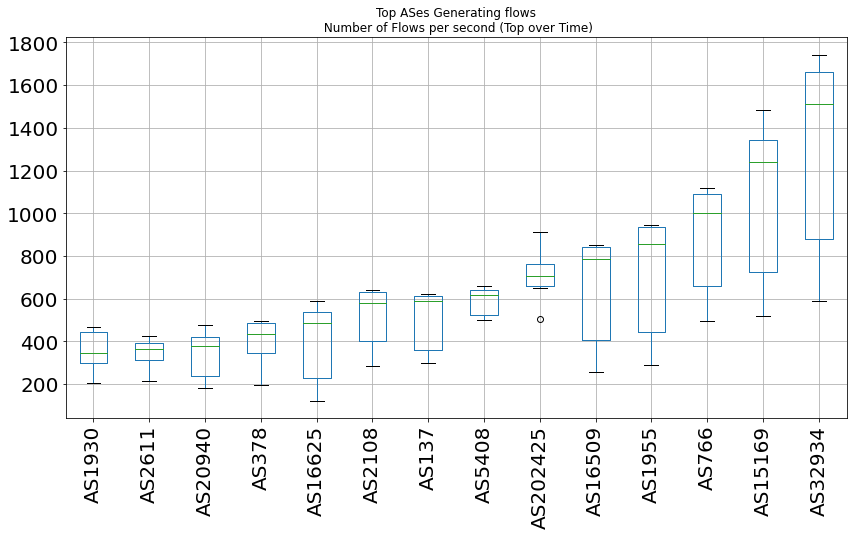
\includegraphics[width=\columnwidth]{img/BCH2_top14AS_generating_fps.png}
          \caption{Top 14 ASes generating flow before new year holidays}
          \label{fig:BCH2_topAS_gen_fps}
    \end{subfigure}
    \begin{subfigure}{\linearFigSze\textwidth}
          \centering
          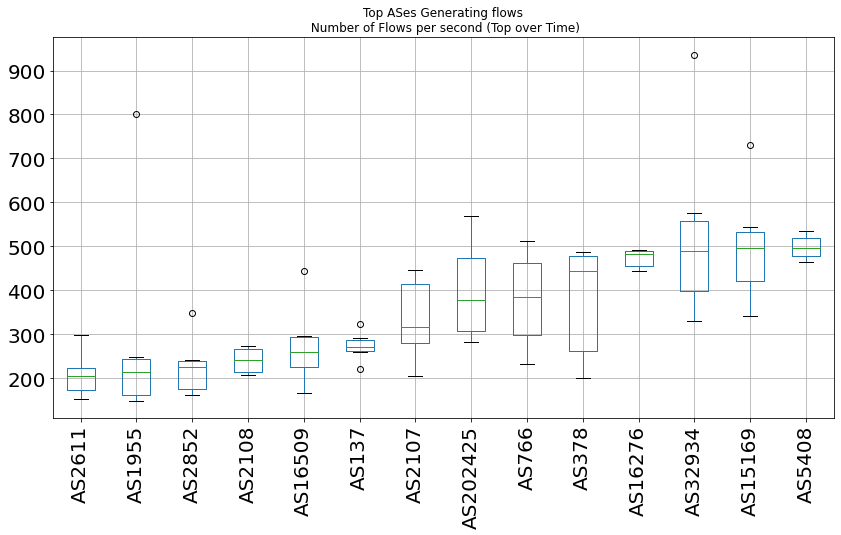
\includegraphics[width=\columnwidth]{img/CH2_top14AS_generating_fps.png}
          \caption{Top 14 ASes generating flow during new year holidays}
          \label{fig:CH2_topAS_gen_fps}
    \end{subfigure}
    \caption{Impact of new year holidays on flow rate of academic and business traffic}
    \label{fig:flowrate_topAS_gen_BCH_CH}
\end{figure}


\begin{figure}
    \begin{subfigure}{\linearFigSze\textwidth}
          \centering
          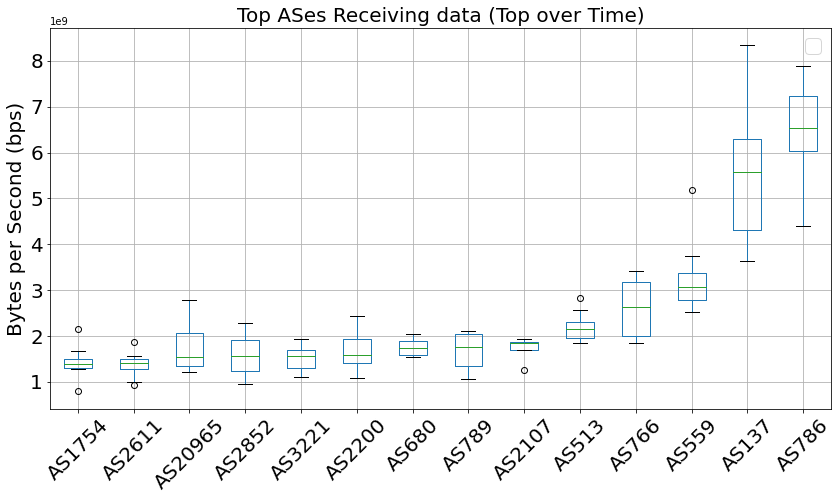
\includegraphics[width=\columnwidth]{img/BCH2_top14AS_recieving_bps.png}
          \caption{Top 14 ASes receiving traffic before new year holidays}
          \label{fig:BCH2_topAS_rec_bps}
    \end{subfigure}
    \begin{subfigure}{\linearFigSze\textwidth}
          \centering
          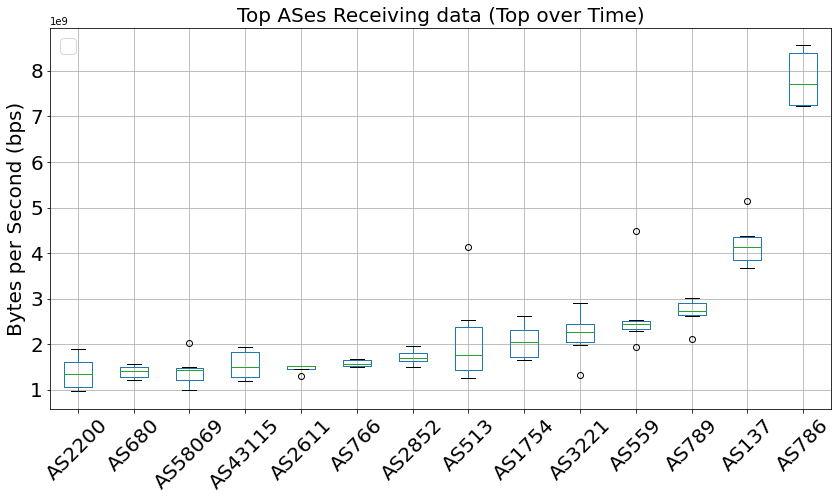
\includegraphics[width=\columnwidth]{img/CH2_top14AS_recieving_bps.png}
          \caption{Top 14 ASes receiving traffic during new year holidays}
          \label{fig:CH2_topAS_rec_bps}
    \end{subfigure}
    \caption{Impact of new year holidays on data rate of academic and business traffic}
    \label{fig:topAS_rec_BCH_CH}
\end{figure}

\begin{figure}
    \begin{subfigure}{\linearFigSze\textwidth}
          \centering
          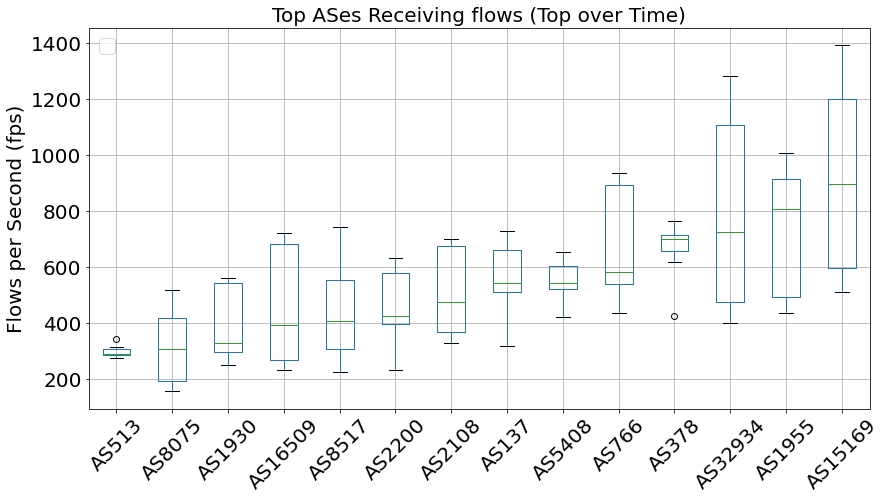
\includegraphics[width=\columnwidth]{img/BCH2_top14AS_recieving_fps.png}
          \caption{Top 14 ASes receiving flow before new year holidays}
          \label{fig:BCH2_topAS_rec_fps}
    \end{subfigure}
    \begin{subfigure}{\linearFigSze\textwidth}
          \centering
          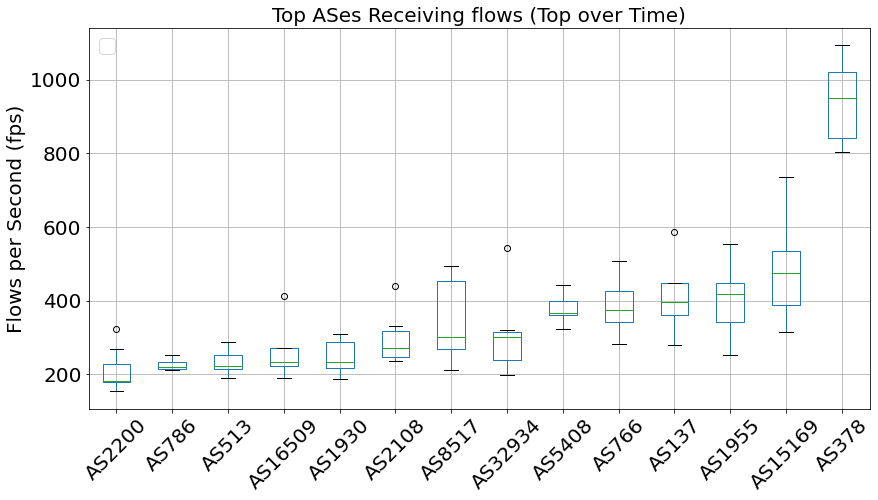
\includegraphics[width=\columnwidth]{img/CH2_top14AS_recieving_fps.png}
          \caption{Top 14 ASes receiving flow during new year holidays}
          \label{fig:CH2_topAS_rec_fps}
    \end{subfigure}
    \caption{Impact of new year holidays on flow rate of academic and business traffic}
    \label{fig:flowrate_topAS_rec_BCH_CH}
\end{figure}




\subsection{Discussion}



\section{Impact of Covid-19 on GEANT}

\subsection{Total Traffic Throughput}
Due to the COVID19 pandemic, traffic in terms of bytes dropped by almost one-third, whereas overall flows dropped by almost half. This difference in observation could be due to the nature of flows. A flow is a unidirectional sequence of packets that contains among other things an ingress interface, IP protocol, source and destination IP addresses, source and destination ports and type of service. While flows require an ingress interface and a request initiating a flow, traffic in bytes may just be machine-to-machine. This is further supported by similar trends during the Christmas/NYE holidays.

\subsection{Academic and Business Traffic}
\begin{figure}
    \begin{subfigure}{\linearFigSze\textwidth}
          \centering
          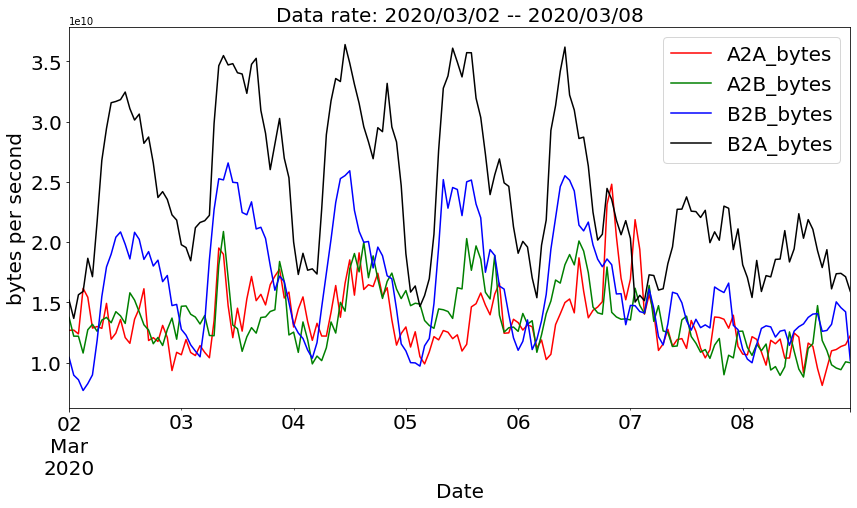
\includegraphics[width=\columnwidth]{img/BCO2_acaBus_bps.png}
          \caption{Data-rate before COVID-19 pandemic}
          \label{fig:BCO2_acaBus_bps}
    \end{subfigure}
    \begin{subfigure}{\linearFigSze\textwidth}
          \centering
          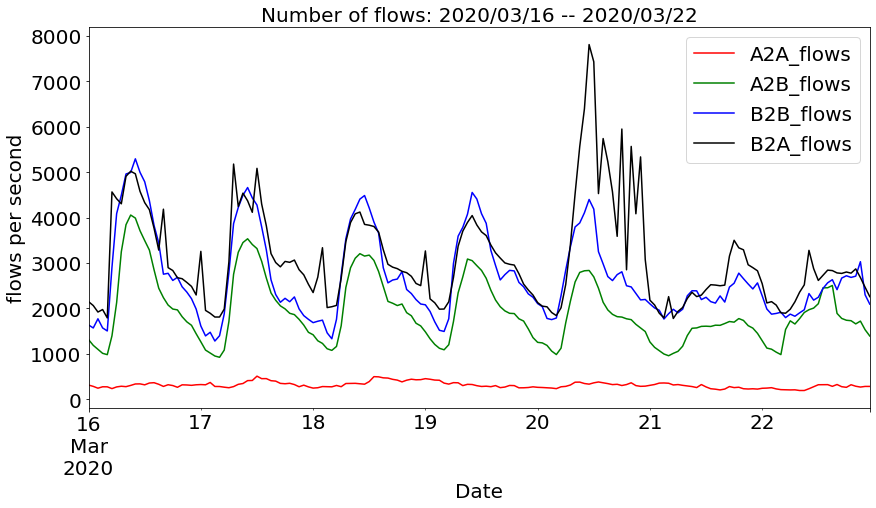
\includegraphics[width=\columnwidth]{img/CO2_acaBus_bps.png}
          \caption{Data-rate during COVID-19 pandemic}
          \label{fig:CO2_acaBus_bps}
    \end{subfigure}
    \caption{Impact of COVID-19 pandemic on data rate of academic and business traffic}
    \label{fig:datarate_acaBus_BCO_CO}
\end{figure}

\begin{figure}
    \begin{subfigure}{\linearFigSze\textwidth}
          \centering
          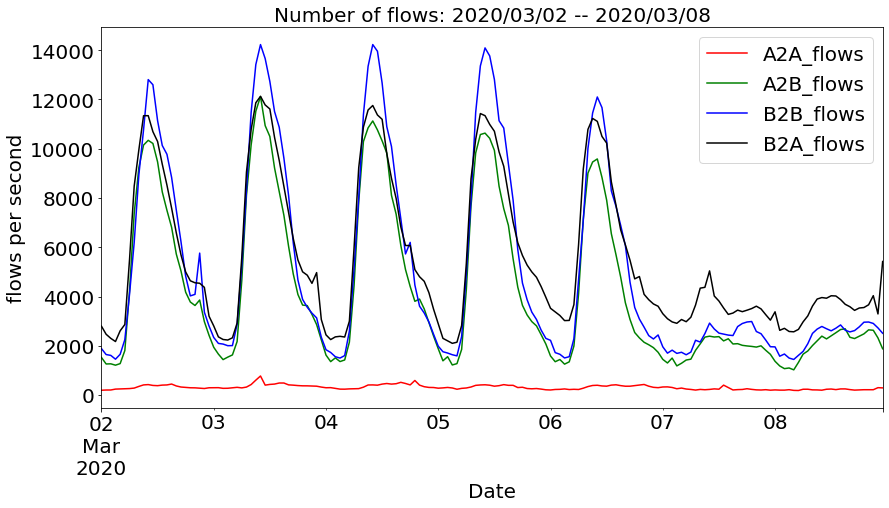
\includegraphics[width=\columnwidth]{img/BCO2_acaBus_fps.png}
          \caption{Flow-rate before COVID-19 pandemic}
          \label{fig:BCO2_acaBus_fps}
    \end{subfigure}
    \begin{subfigure}{\linearFigSze\textwidth}
          \centering
          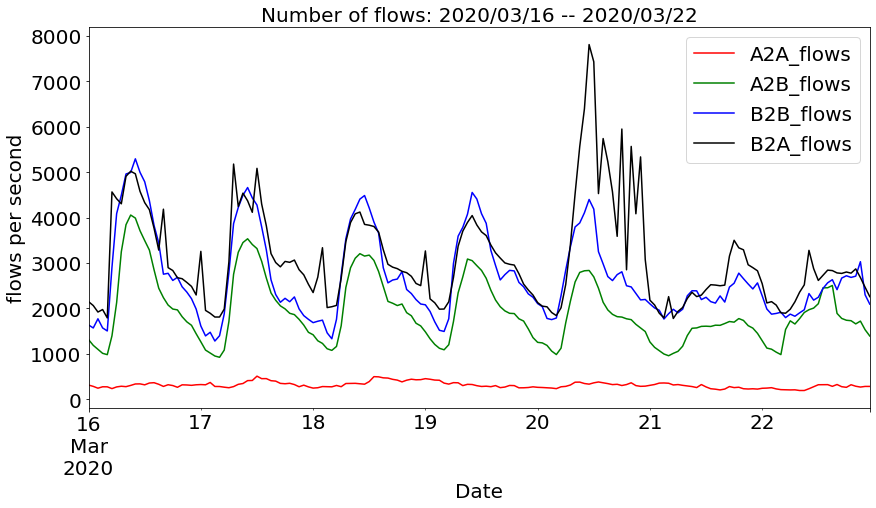
\includegraphics[width=\columnwidth]{img/CO2_acaBus_fps.png}
          \caption{Flow-rate during COVID-19 pandemic}
          \label{fig:CO2_acaBus_fps}
    \end{subfigure}
    \caption{Impact of COVID-19 pandemic on flow rate of academic and business traffic}
    \label{fig:flowrate_acaBus_BCO_CO}
\end{figure}
\subsection{NRENs Traffic}

\subsection{Top ASes}

\begin{figure}
    \begin{subfigure}{\linearFigSze\textwidth}
          \centering
          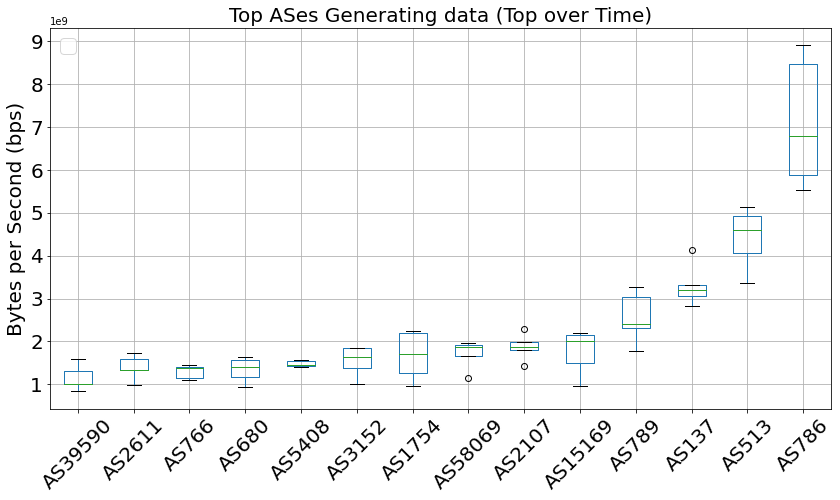
\includegraphics[width=\columnwidth]{img/BCO2_top14AS_generating_bps.png}
          \caption{Top 14 ASes generating traffic before COVID-19 pandemic}
          \label{fig:BCO2_topAS_gen_bps}
    \end{subfigure}
    \begin{subfigure}{\linearFigSze\textwidth}
          \centering
          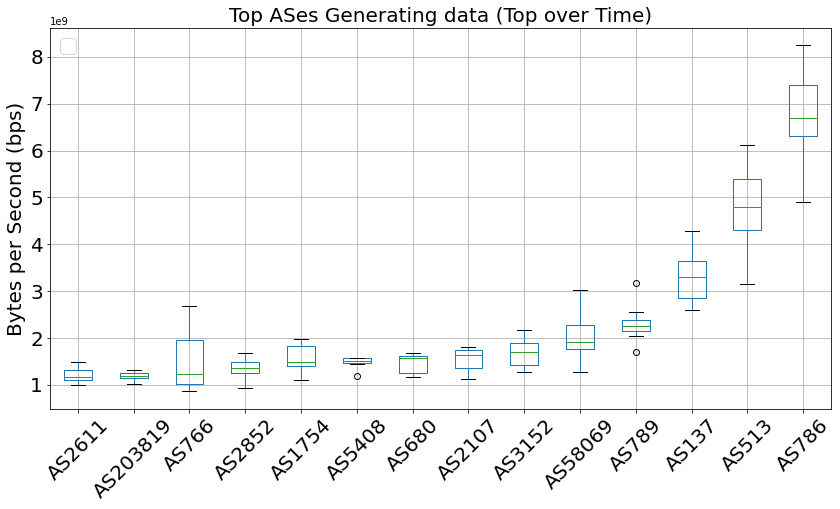
\includegraphics[width=\columnwidth]{img/CO2_top14AS_generating_bps.png}
          \caption{Top 14 ASes generating traffic during COVID-19 pandemic}
          \label{fig:CO2_topAS_gen_bps}
    \end{subfigure}
    \caption{Impact of COVID-19 pandemic on data rate of academic and business traffic}
    \label{fig:topAS_gen_BCO_CO}
\end{figure}

\begin{figure}
    \begin{subfigure}{\linearFigSze\textwidth}
          \centering
          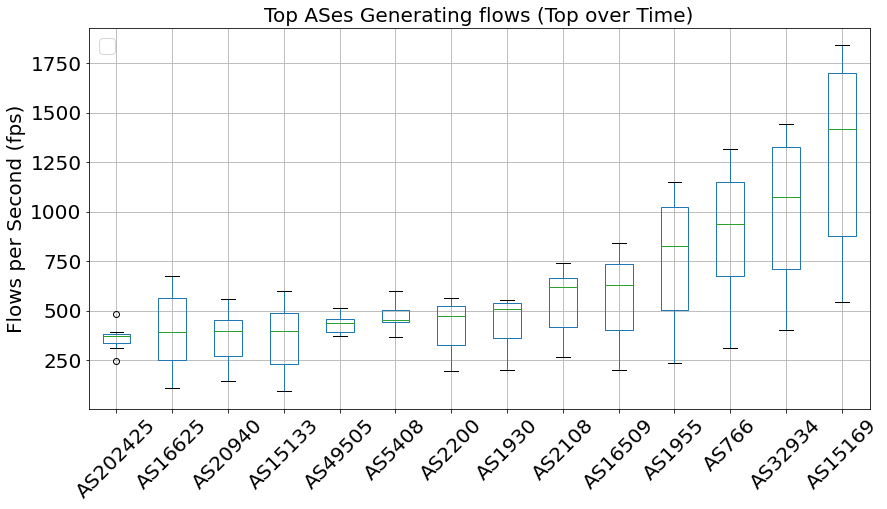
\includegraphics[width=\columnwidth]{img/BCO2_top14AS_generating_fps.png}
          \caption{Top 14 ASes generating flow before COVID-19 pandemic}
          \label{fig:BCO2_topAS_gen_fps}
    \end{subfigure}
    \begin{subfigure}{\linearFigSze\textwidth}
          \centering
          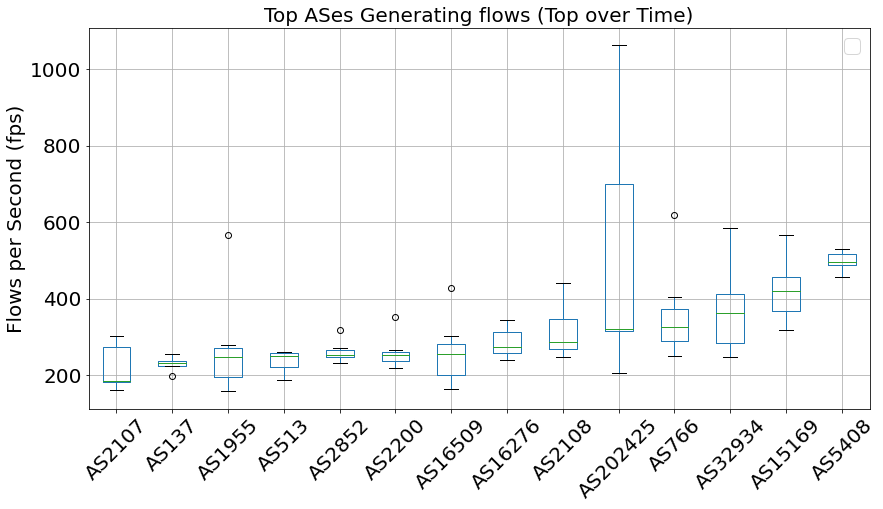
\includegraphics[width=\columnwidth]{img/CO2_top14AS_generating_fps.png}
          \caption{Top 14 ASes generating flow during COVID-19 pandemic}
          \label{fig:Co2_topAS_gen_fps}
    \end{subfigure}
    \caption{Impact of COVID-19 pandemic on flow rate of academic and business traffic}
    \label{fig:flowrate_topAS_gen_BCO_CO}
\end{figure}


\begin{figure}
    \begin{subfigure}{\linearFigSze\textwidth}
          \centering
          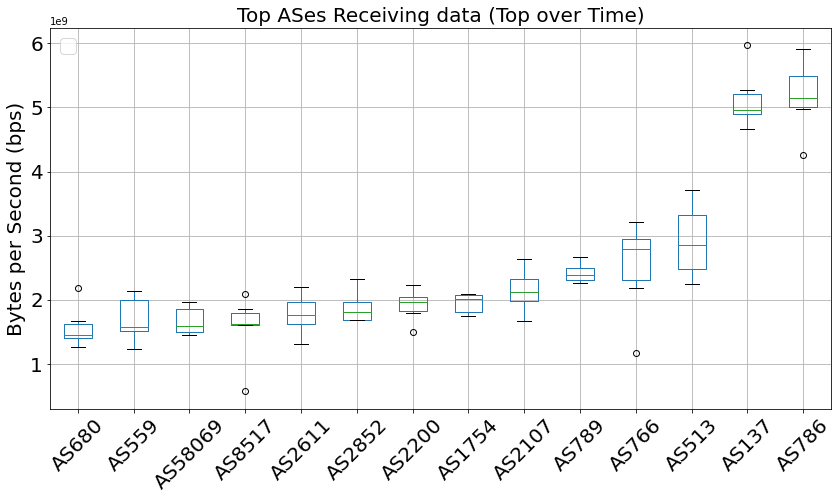
\includegraphics[width=\columnwidth]{img/BCO2_top14AS_recieving_bps.png}
          \caption{Top 14 ASes receiving traffic before COVID-19 pandemic}
          \label{fig:BCO2_topAS_rec_bps}
    \end{subfigure}
    \begin{subfigure}{\linearFigSze\textwidth}
          \centering
          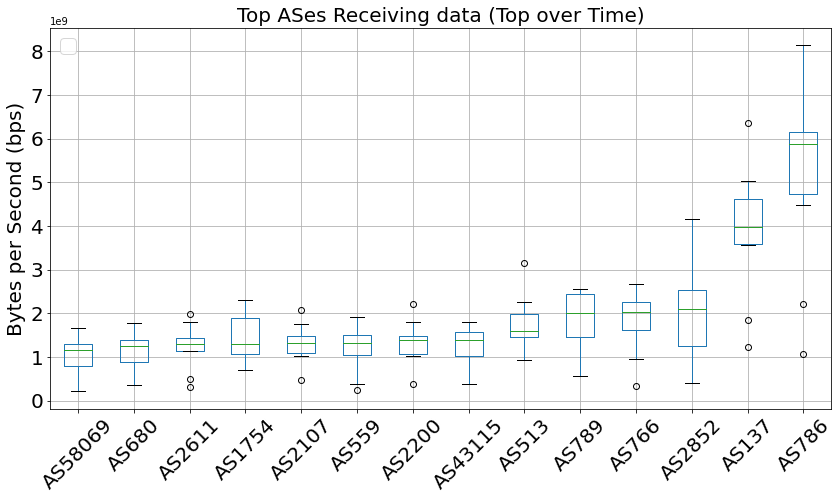
\includegraphics[width=\columnwidth]{img/CO2_top14AS_recieving_bps.png}
          \caption{Top 14 ASes receiving traffic during COVID-19 pandemic}
          \label{fig:CO2_topAS_rec_bps}
    \end{subfigure}
    \caption{Impact of COVID-19 pandemic on data rate of academic and business traffic}
    \label{fig:topAS_rec_BCO_CO}
\end{figure}

\begin{figure}
    \begin{subfigure}{\linearFigSze\textwidth}
          \centering
          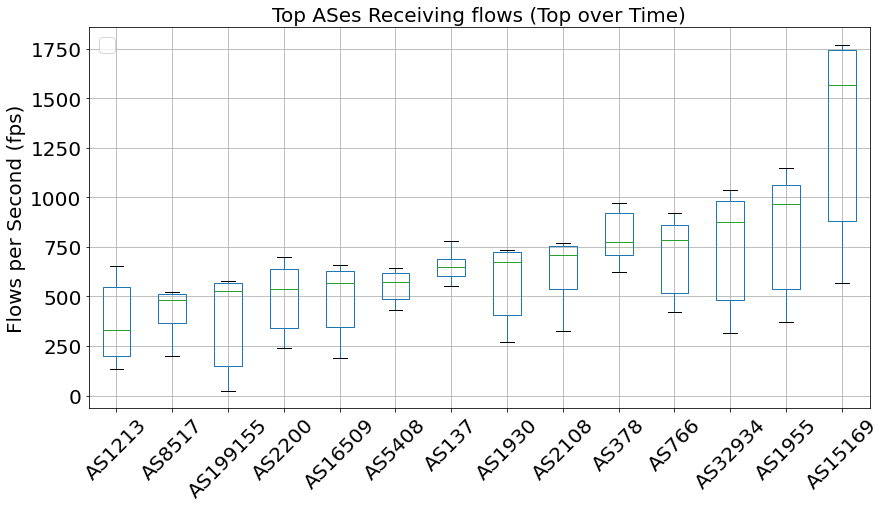
\includegraphics[width=\columnwidth]{img/BCO2_top14AS_recieving_fps.png}
          \caption{Top 14 ASes receiving flow before COVID-19 pandemic}
          \label{fig:BCO2_topAS_rec_fps}
    \end{subfigure}
    \begin{subfigure}{\linearFigSze\textwidth}
          \centering
          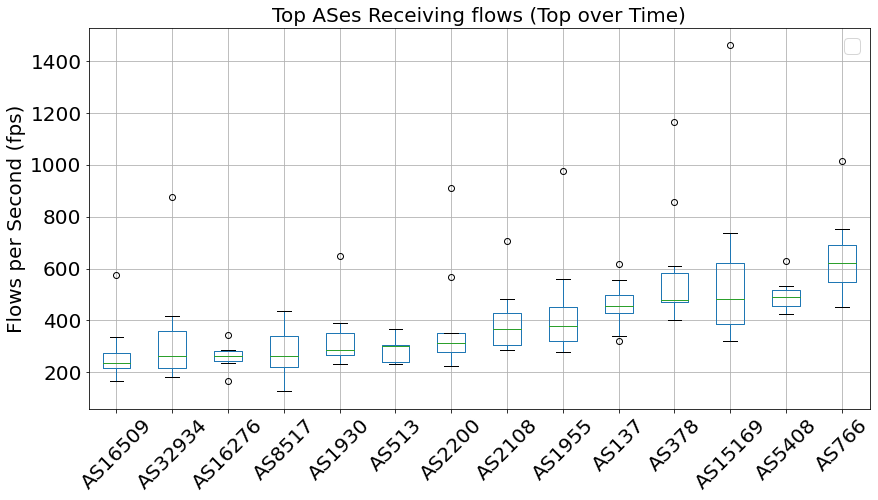
\includegraphics[width=\columnwidth]{img/CO2_top14AS_recieving_fps.png}
          \caption{Top 14 ASes receiving flow during COVID-19 pandemic}
          \label{fig:CO2_topAS_rec_fps}
    \end{subfigure}
    \caption{Impact of COVID-19 pandemic on flow rate of academic and business traffic}
    \label{fig:flowrate_topAS_rec_BCO_CO}
\end{figure}
\subsection{Discussion}

\section{Comparing Covid-19 and New Year Holidays impact on GEANT}




\section{OLD PARTS}
\subsection{Sankey Plot}
In these plots, the top-n one-way communications are considered. For example, consider

A->B: 10 bps (meaning that there is a traffic flow of 10 bps from A to B)
A->C: 1 bps
A->D: 9bps
B->C:11bps
B->D: 3bps
B->A:5bps
then the top-3 one-way communications are:
A->B:10bps
A-D:9bps
B-C:11bps

AS-Level Analysis: every AS is considered as a unique entity. Each NREN has one or more AS-number. Each of these numbers are considered as one unique entity.

NREN-Level Analysis: all ASes belonging to an NREN are aggregated together, e.g., consider AS7 is in customer cone of AS786 (JISC). The traffic generated by AS7 and destinated to AS-x (AS7 -> AS-x) will be considered as AS786 -> AS-x. Besides, if there are more than one ASN assigned to an NREN, these ASNes would be aggregated into one, e.g., if AS786 and AS133084 are both assigned to JISC then we replace AS133084 with AS786 everywhere.



\subsection{ASes}

\red{For top ASes we will need to know the overlap (i.e. common ASes) for measurement criteria. That is, how many top ASes in terms of generating traffic measured in bps are in the top ASes list if measured in terms of fps. And vice versa, e.g. receiving traffic in bps and fps, etc.}

\subsubsection{Top ASes fps and bps (box plot)}
In the following, top ASes are specified. The approach used to specify the top ASes is 'top over time': average the total output of each AS during the sampling period, and select the top x ASes.
Each AS may generate traffic or receives traffic, therefore, plots are divided into two categories 'Top ASes Generating Traffic' and 'Top ASes Receiving Traffic'.

\end{document}
